\documentclass[a4paper, 12pt]{report}
\usepackage[utf8]{inputenc}
\usepackage{biblatex}
\usepackage{gnuplottex}
\usepackage{graphicx}
\graphicspath{ {./Pictures/} }
\usepackage{lscape}
\usepackage[english,russian]{babel}
\usepackage{epsfig}
\usepackage{verbatim}
\usepackage[left=2cm, right=1cm, top=2cm, bottom=2cm]{geometry}
\usepackage{listings}
\usepackage{setspace}
\usepackage{pdflscape}
\usepackage{xcolor}

\definecolor{codegreen}{RGB}{46, 198, 66}
\definecolor{codegray}{RGB}{193, 185, 195}
\definecolor{backcolour}{RGB}{246, 18, 255}
\definecolor{codered}{RGB}{240, 17, 17}

\lstdefinestyle{mystyle}{
    backgroundcolor=\color{backcolour},   
    commentstyle=\color{codegreen},
    keywordstyle=\color{magenta},
    numberstyle=\tiny\color{codered},
    stringstyle=\color{backcolour},
    basicstyle=\ttfamily\footnotesize,
    breakatwhitespace=false,         
    breaklines=true,                 
    captionpos=b,                    
    keepspaces=true,                 
    numbers=left,                    
    numbersep=5pt,                  
    showspaces=false,                
    showstringspaces=false,
    showtabs=false,                  
    tabsize=2
}

\lstset{style=mystyle}
\usepackage{hyperref}
\hypersetup{
    colorlinks=true,
    linkcolor=blue,
    filecolor=magenta,      
    urlcolor=red,
    pdfpagemode=FullScreen,
    }
\onehalfspacing

\title{"PC Engine" - the greatest technical adventure}
\author{Efremov Evgeni Yurievich}
\date{February 2026}
\begin{document}

\maketitle
\begin{abstract}
\color{white}
\colorbox{red}{Тема: историческое исследование домашней игровой консоли}
\color{black}
\newlineКлючевые слова: PC Engine, $CD-ROM^2$, Hudson Soft, NEC
\end{abstract}

\tableofcontents
\newpage

\chapter{Введение}
\begin{figure}
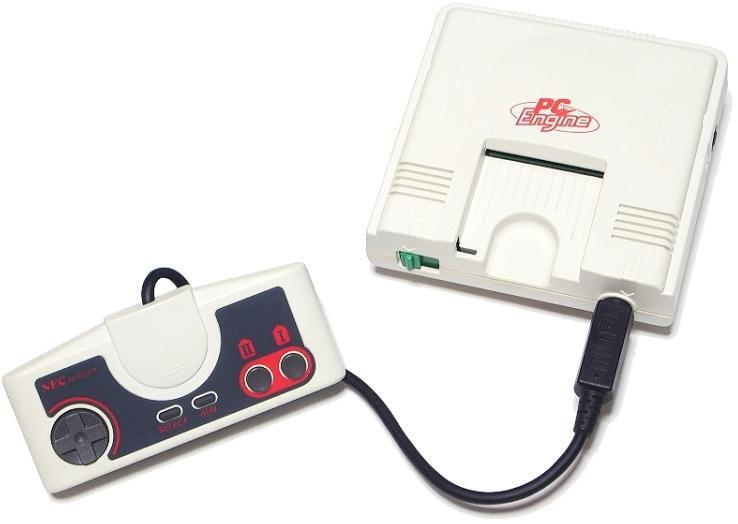
\includegraphics[width = 0.5\textwidth]{images/PC_ENGINE.jpg}
\end{figure}
В октябре 1987 года компании Hudson Soft и NEC представили домашнюю игровую систему PC Engine - компактное и мощное устройство с революционной моделью развития. На старте консоль уже била рекорды: продукт был включён в книгу рекордов Гиннеса как самая компактная игровая система, при этом по мощности\footnote{Характеристики устройства представлены в отдельном разделе на странице 3\pageref{third}.} она ничуть не отставала от главенствующего игрока на рынке того времени - Nintendo Famicom. Первоначально носителем данных были выбраны картриджи в форм-факторе компактных карточек - HuCard, размер хранимых данных на которых изначально составлял 256Кб и в дальнейшем был расширен до 24Мб с помощью технологии переключения банков памяти. Но сама консоль была всего лишь ядром целой экосистемы устройств, выпущенных компаниями за долгие 12 лет жизненного цикла системы. Среди них были CD-ROM привод, с помощью которого консоль могла воспроизводить программы с компакт-дисков формата Audio CD, CD+G, $CD-ROM^2$ и $Super CD-ROM^2$ (последние два формата - уникальные разработки программистов из Hudson). Также были выпущены модули энергонезависимой памяти для сохранений прогресса, портативные модели PC Engine GT, как отдельное устройство в отличном корпусе, и PC Engine LT, как модификация стандартной PC Engine со встроенным экраном, с TV-тюнером, возможностью совместной игры при помощи аксессуара "COM Cable" и совместимостью с большинством аксессуаров и многое другое.

\begin{landscape}

\pagecolor{black}
\color{white}
\chapter{Технические Характеристики}
Технические Характеристики
\begin{enumerate}
\item Процессор - 8-битный MOS Technology 65SC02 (также имеющий название HuC6280 от Hudson) — 8-битные регистры и шина данных, 16-битная адресная шина и счетчик. Частота CPU 1.79 или 7.16 МГц (выбирается программно).
\item Видео
\begin{itemize}
    \item Видеосистема: два 16-битных процессора — HuC6270 и HuC6260.
    \item Разрешение экрана: 256 x 216 пикселей.
    \item Спрайты: до 64, размером от 16x16 до 32x64, 16-цветные.
    \item Цветов на экране: 512 — (256 для спрайтов и 256 для фона).
    \item Видеопамять: 64 Кб (для TurboDuo: 512Кб)
\end{itemize}
\item Звук
\begin{itemize}
    \item Звуковой процессор: 8 бит PCM стерео / 6-канальное стерео.
\end{itemize}
\item Оперативная память - 8 Кбайт.
\item Носители
\begin{itemize}
    \item Ёмкость картриджа: от 256 килобайт до 24 мегабайт.
\end{itemize}
\item Привод CD-ROM - Скорость 1x (в качестве отдельного адд-она к приставке)
\end{enumerate}
\end{landscape}

\pagecolor{white}
\color{black}
\chapter{Хронология выпуска устройств}
Хронология выпуска устройств (Япония)\newline

\begin{tabular}{|c|c|} 
 \hline
 Устройство & Дата выхода \\
 \hline \hline
 PC Engine  & 30.10.1987  \\
 \hline
 PC Engine $CD-ROM^2$ & 4.12.1988 \\
 \hline
 PC Engine Shuttle & 22.11.1989 \\
 \hline
 PC Engine CoreGrafx & 8.12.1989 \\
 \hline
 PC Engine SuperGrafx & 8.12.1989 \\
 \hline
 PC Engine GT & 1990 \\
 \hline
 PC Engine Duo & 21.09.1991 \\
 \hline
 PC Engine LT & 13.12.1991 \\
 \hline
 PC Engine Duo-R & 1993 \\
 \hline
 PC Engine Duo-RX & 1994 \\
 \hline
\end{tabular}
\newline

Хронология выпуска устройств (США)\newline

\begin{tabular}{|c c|c|} 
 \hline
 Устройство & Аналог в Японии & Дата выхода \\
 \hline \hline
 TurboGrafx-16 & PC Engine  & 29.08.1989  \\
 \hline
 TurboGrafx-CD & PC Engine $CD-ROM^2$ & 1990 \\
 \hline
 Turbo Express & PC Engine GT & 1990 \\
 \hline
 Turbo Duo & PC Engine Duo & 21.09.1991 \\
 \hline
\end{tabular}
\newline

С полной хронологией выпуска устройств и аксессуаров вы можете ознакомиться \href{https://pcengine.ru/history-of-consoles-pc-engine-turbografx-16/}{ЗДЕСЬ}

\newpage
\chapter{ОФФТОП-1: Фрагменты кода}
\lstinputlisting[language=Python, firstline=3, lastline=35]{main_2.py}
\newpage
\lstinputlisting[language=C++, firstline=6]{task_A.cpp}
\newpage
\chapter{ОФФТОП-2:Формула Тейлора}
Формула Тейлора дает представление функции в виде\newline
$f(x) = f_0(x)+f_1(x)+...,$

где $f_k(x^1, ...,x^n)$ - функция степени k от переменных $(x^1, ...,x^n)$.\newline
Добавление каждой новой функции $f_k$ — это более точная аппроксимация функции f.\newline
График Г функции f — это гиперповерхность.\newline
\begin{equation}
\Gamma_f=\lbrace(x, f(x))\rbrace=\lbrace(x^1,...,x^n,f(x^1,...,x^n))\rbrace\in R^{n+}
\end{equation}
Она складывается из графиков функций $f(x_0),f_1,f_2,...$.
График функции
\begin{equation}
f(x_0) + f_1(x) = f(x_0)+\Sigma_{i=1}^n\frac{\delta f}{\delta x^i}(x_0)(x^i-x^i_0)
\end{equation}

обозначается $T_{x_0}$.\newline
Таким образом, уравнение плоскости $T_{x_0}$ в координатах $(x^1,...,x^n,z)$ имеет вид
\begin{equation}
z=f(x_0)+\Sigma_{i=1}^n\frac{\delta f}{\delta x^i}(x_0)(x^i-x^i_0)
\end{equation}
\bfТеорема 7.1.\it Плоскость $T_{x_0}$ совпадает с касательной плоскостью, т.е. состоит из всех точек вида $(x_0, f(x_0))+\nu$, где $\nu$ - касательный вектор к некоторой линии на графике $\Gamma_i$ в точке $(x_0, f(x_0))$.
\newline \ttД о к а з а т е л ь с т в о. \rm Если $(x(t), f(x(t)))$ - произвольная линия на графике, с началом в точке $x(0) = x_0$, то касательный вектор имеет вид\newline

\chapter{ОФФТОП-3: Графики функций}

\begin{figure}[h]
 \centering
 \begin{gnuplot}
  set title "Явная функция одной переменной"
  set terminal epslatex color size 12cm,15cm
  set xlabel "X"
  set ylabel "Y"
  set xzeroaxis lt -1
  set yzeroaxis lt -1
  set style line 1 lt 1 lw 4 lc rgb '#4682b4' pt -1
  set grid ytics lc rgb '#555555' lw 1 lt 0
  set grid xtics lc rgb '#555555' lw 1 lt 0
  set xrange [-3:3]
  plot x**3 title '$y = x^3$' ls 1	
 \end{gnuplot}
\end{figure}

\begin{figure}[h]
    \centering
    \begin{gnuplot}
        set title "Параметрическое представление кривой"
        set terminal epslatex color size 12cm,15cm
        set xzeroaxis lt -1
        set yzeroaxis lt -1
        set style line 1 lt 1 lw 4 lc rgb '#4682b4' 
        set grid ytics lc rgb '#555555' lw 1 lt 0
        set grid xtics lc rgb '#555555' lw 1 lt 0
        set size ratio 1
        set xlabel "X"
        set ylabel "Y"
        set parametric
        plot sin(t),cos(t) with lines
    \end{gnuplot}
\end{figure}

\begin{figure}[h]
    \centering
    \begin{gnuplot}
        set title "Представление кривой в полярных координатах"
        set terminal epslatex color size 12cm,15cm
        set polar
        set grid polar
        unset key
        set samples 300
        set xrange [0:2*pi]
        set yrange [-pi:pi]
        plot 3*cos(5*t), 3*cos(3*t) ls 3,1
    \end{gnuplot}
\end{figure}

\begin{figure}[h]
    \centering
    \begin{gnuplot}
        set terminal epslatex color size 12cm,15cm
        set title "Сферические координаты"
        set mapping spherical
        set parametric
        set xlabel "X"
        set ylabel "Y"
        set zlabel "Z"
        splot cos(u)*cos(v), cos(u)*sin(v), sin(u)
    \end{gnuplot}
\end{figure}

\begin{figure}[h]
    \centering
    \begin{gnuplot}
        set terminal epslatex color size 12cm,15cm
        set title "Цилиндрические координаты"
        set mapping cylindrical
        set parametric
        set xlabel "X"
        set ylabel "Y"
        set zlabel "Z"
        splot cos(u), sin(u), v
    \end{gnuplot}
\end{figure}

\end{document}